\chapter{Methodology}
% information on the corpus and writing data
%define  features that I will use for classification how I decided on this and motivation behind these features.
\section{Characteristics of Japanese}
The agglutinative nature of Japanese coupled with the absence of explicit word delimiters, presents challenges for
accurate word segmentation. Furthermore, the use of three distinct writing systems
\footnote{Hiragana, Katakana, and Kanji} leads to considerable orthographic variation. for instance, learners at
lower proficiency levels frequently rely on the phonetic alphabets (hiragana and katakana), which can exacerbate
segmentation and tokenization errors. This phenomenon has been observed in previous studies
\citep{yang1998, nagata2009}, where systems demonstrated a lack of robustness against "spelling" errors or the
erroneous use of kanji.

Defining a "word" in Japanese also differs considerably from Indo-European languages. While a bound morpheme in
Enlgish might be treated as a indificual word. this is generally not the case in Japanese. For example,
segmentation can be difficult.
With 3
alphabets used there can orthographic variation is also fairly common. Learners at the lower proficentcy levels
mostly will write using the phonetic alphabets hiragana and katakana sometimes leading to errors in
segmentation/tokenization as was observed in \citep{yang1998, nagata2009}.

What is considered a word in Japanese may differ from other languages european languages. While a bound morpheme in
English might be treated
as an individual word, this is generally not the case in Japanese. For example, the word 話す\textit{hanasu}(to speak)
is considered a single word. However its potential form, 話せる \textit{hanaseru}(to be able to speak) is often analyzed as
two distinct morphemes: 話\textit{hana} and せる\textit{seru}. Initial abalyses using the chose tokenizer and parser
revealed inconsistencies in this regard. Similar inconsistencies were observed with compound verbs, such as
言い切る(\textit{iikiru}, "to completely say\footnote{\textit{to say without restraint}}"). While this was consistently
split into 言い(\textit{ii}"to say") and 切る(\textit{kiru} a suffix indicating completion), other instances were
segmented into
食べ (\textit{tabe}"to eat") 切る(\textit{kiru}"completely"). These inconsistencies pose significant hurdles for the
reliable extraction of specific grammatical forms for criterial features and can lead to unreliable counts for
complexity measures.
% maybe say something about taking this into consideration when writing rules for criterial features.

\section{About the International Corpus of Japanese as a Second Language(I-JAS)}
information about the IJATS corpus organization

This study utilizes data from the International Corpus of Japanese as a Second Language (I-JAS), as
detailed in
\citet{Sakoda2020}, was
used.  The
I-JAS corpus is comprised of both spoken and written samples of Japanese.  It includes data from a diverse pool of 1,
000 adult learners
(aged
between 17 and 63 years old), all of whom are learning Japanese as a second language. 50 Native speaker samples are also
included in the corpus as a control group.

Participant's proficiency levels were assessed using the Japanese Computer Adaptive Test (J-Cat)
\citep{Imai2009}, with Further details about this assessment is provided in the
subsequent
section \ref{j-cat}. In addition to proficiency scores, the corpus includes various metadata for each participant,
such as
their
native language,
prior experience of visiting or living in Japan, and current geographical location (whether outside or within Japan).

%%%%%%% This part below contains information only on the essay writing samples I previously analyzed. I have also
%%%%%%% included additional writing samples added to the corpus which has brought the total particiapnt pool to 1000
%%%%%%% again.
Writing samples were extracted from the larger I-JAS corpus. Samples  were provided from 687 individuals, including the
control group
of 50 native speakers. A detailed breakdown of the of the participants in the writing sample subset, categorized by
their corresponding Japanese Language Proficiency Test (JLPT) levels, is presented in \ref{tab:participants-chart}.

%Name: count, dtype: int64
\begin{table}
\centering
\begin{tabular}{cc}
\hline \textbf{JLPT Proficiency Level} & \textbf{\# of Participants} \\ \hline
N5 & 176 \\
N4  & 318 \\
N3 & 297\\
N2 & 165 \\
N1 & 44 \\
Native Speakers & 50 \\
\hline
\end{tabular}
\caption{\label{tab:participants-chart} Distribution of participants across JLPT proficiency levels. J-cat scores have been mapped to their equivallent JLPT levels. }
\end{table}


\subsection{J-CAT test}
\label{j-cat}

%background and information on the J-CAT test compare to JLPT.

The Japanese Computerized Adaptive Test (J-CAT) \citep{Imai2009}, is a computer-administered assessment
designed to evaluate an
individual's proficiency in the Japanese language. While formerly freely accessible, the J-CAT is now overseen by
the  日本語教育支援協会(Japanese Language Education Support Association (JaLESA)). Japanese
universities frequently
employ the J-CAT as an efficient tool and flexible tool for placing foreign students into appropriate Japanese
language courses, primarily due to its on-demand administration compared to the JLPT which is only
administered bi-annually.

This adaptive test tailors its
question difficulty to a
student's performance in
the areas of Vocabulary, Grammar, Listening, and Reading.

\begin{figure}[h]
    \centering
    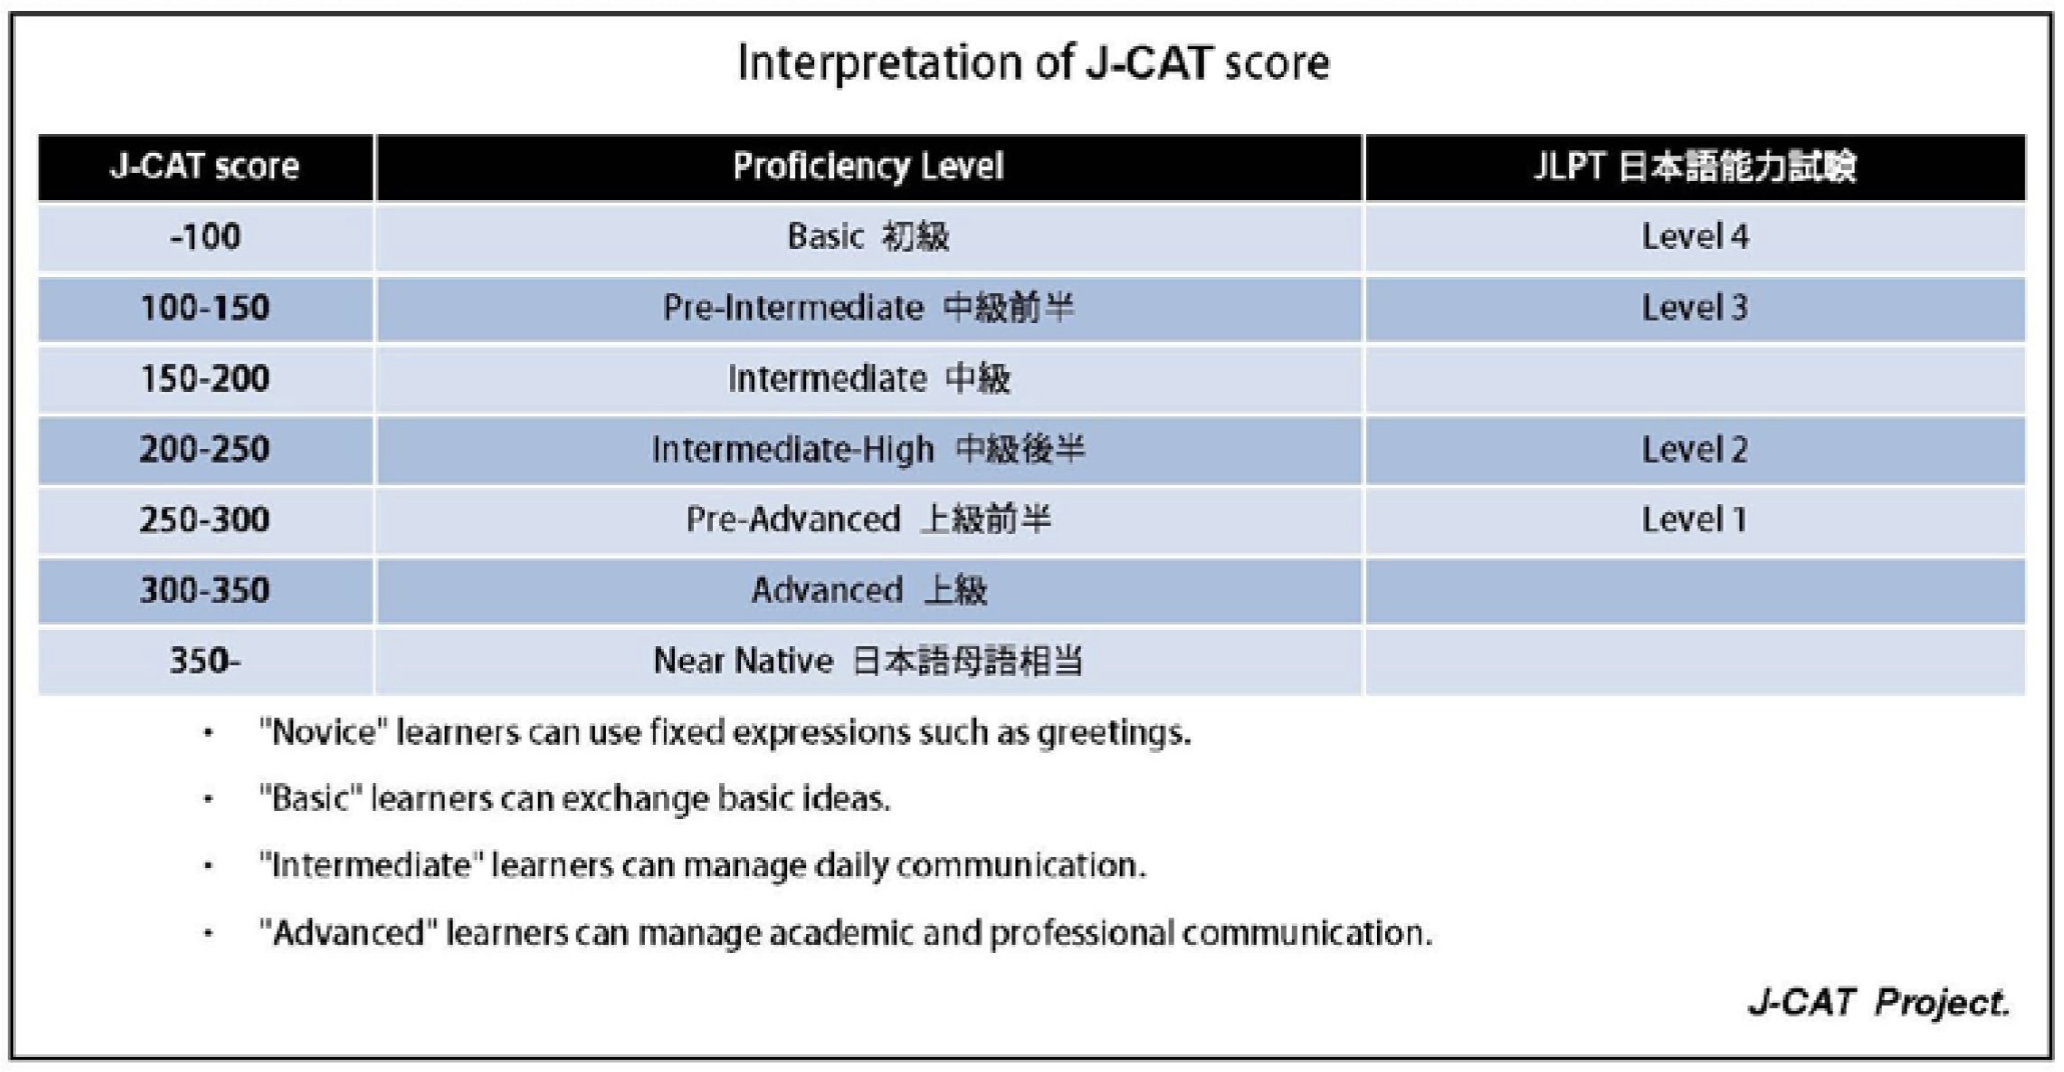
\includegraphics[scale=.3]{img/JCatScores.png}
    \caption[J-Cat Proficency Levels]{The assigned proficency levels from the J-Cat test as taken from the original paper in  2009. Please note that the given JLPT levels do not correspond to the current JLPT test which was reformed in 2010. A new score interpretation connecting JLPT levels to J-Cat scores was released in 2011 and is shown in Table \ref{tab:proficency-table} }
    \label{fig:JCatLevels}
\end{figure}

Each student receives a numerical score that corresponds to one of seven distinct proficiency levels, as detailed in
Table \ref{tab:proficency-table}. These proficency levels have also been mapped to an equivallent Japanese Language
Proficency
Test(JLPT) score.
This study will categorize
participants according to their JLPT level. Participants in the
native speaker control group were given a default J-cat score of 999.

\begin{table}
\centering
\begin{tabular}{lrl}
\hline \textbf{JLPT Proficiency Level} & \textbf{J-Cat Score}  \\ \hline
N5 & 0 - 149 \\
N4 & 150 - 199 \\
N3 & 200 - 249 \\
N2 & 250 - 299 \\
N1 & 300 - \\
Native & 999
\hline
\end{tabular}
\caption[Proficency Levels]{JLPT proficency level classification based on J-cat score taken from
\cite{jcat_interpretation_guide}.}
\label{tab:proficency-table}
\end{table}

\subsection{Writing Tasks}

% add the additional SW 1 and 2 tasks where participants were expected to write a story based on a picture.
Each participant submitted four samples of writing for specific tasks:
\begin{itemize}
    \item A short essay titled "Our Eating Habits" involving a comparison between fast food and home-cooked meals in the learner's home country.
    \item A letter addressed to a former teacher, requesting a letter of recommendation for a scholarship application.
    \item An email seeking an extension for the deadline of a report submission.
    \item An apology email in which the learner must decline an invitation.
\end{itemize}
These tasks were consistent across all participants, regardless of their proficiency levels, and encompassed various
task types. The inclusion of a range of task types and formalities was intended to encourage diverse responses from
the students and possibly mitigate a potential "task effect" similar to what  was described in \cite{Alexpoulou2017}.
The writing samples were processed-as-is without being corrected for learner errors.

\subsection{Text Preprocessing}
Mention the preprocessing of the text. Talk about spacys' ginza pipeline used for parsing-tagging etc.
The text of each writing
%% Revise below to explain in more detail the processing of the text... POS, Dependency parsing, Pronunciation,
%% lemmatization.... punctuation was removed for some of the morphological measures
Spacy's Ginza package \cite{Ginza} (v 5.2) for Japanese was utilized to process the corpus texts, given the
absence of existing tools for the analysis of Japanese learner text. The algorithms for calculating various complexity measures were developed by the author of this study\footnote{Code is available at the following github page:  \href{https://github.com/meghorikawa/JFE}{https://github.com/meghorikawa/JFE} }.

\section{Complexity Measures}
detail the complexity measures I will use, how I developed the scripts to automatically "extract them" and the statistical significance between the proficiency levels
list, Sent Length, Clauses per sentence, Noun phrase length,  Subordination, coordination, noun phrase length, MTLD,Morphological complexity? , ADD measures?

lexical sophistication measures use this corpus: \cite{BCCWJ_List} and article citation: \cite{maekawa2014}, Think
about the Tsukuba web corpus also...
When implementing LFP punctuation is removed from the text. Need to mention how text is tokenized in japanese: in
the freq list ばいい is written but would be tokenized as ば and いい ...how to overcome this? Remove verbs? should I use
tokenizer to split the verbs in the word list??

mention the difficulties in finding clauses - specifically in discriminating between coordinate and subordinate
automatically.  POS label SCONJ for subordinate conjunction is used even in the case of coordination, therefore
other methods are needed.

\section{Criterial Features}
Describe the rule based feature matcher I made for extracting certain grammar patterns to disconcern their use
across proficiency levels. Mention how many grammar points at each level I was able to include. Use of the lower
levels doesn't disconcern much so focus should be on the intermediate and upper levels.  Forms that are mainly form
based(and therefore easier to pattern match) should be given priority over. Give some examples of rules derrived

mention that I chose forms which spanned multiple levels. I.e. しか at N4 used with Nouns and しか〜ないat N3 used
with verbs to see if their use at the different levels actually follows this.

don't forget about implementing normalization.

Official documents with grammar from the different levels of JLPT do not exist however many 'unoffical lists' of
grammar, vocabulary, Kanji are available - including Jisho.org, personally compared againast published material from
ARUKU

\section{EBMS}
 Overview was already done in Background section. Mention more details about training etc.


